\chapter{Case Study and Related Work}
\label{chapter-background}

This chapter first presents a case study describing an application that we
have studied in detail: volcano monitoring. We have built several generations
of sensor networks designed to study eruptive activity at volcanos and
deployed them in Ecuador. The second portion of this chapter reviews other
efforts to build the scientific macroscope using sensor network technology.

\section{Case Study: Volcano Monitoring}

Beginning in 2004, computer scientists from Harvard University joined forces
with seismologists from the University of New Hampshire, the University of
North Carolina, and Instituto Geof\'{i}sico, Escuela Polit\'{e}cnica
Nacional, Ecuador, to begin a collaboration aimed at using sensor networks to
further the study of active volcanoes. From a simple starting point --- a
handful of nodes streaming continuous data from a single sensor per node ---
we have developed a sophisticated resource-aware architecture carefully
balancing the value of the data to the application against the network-wide
cost of extraction. These design changes were motivated by the science goals,
responsive to changing hardware platforms, and driven by experience gained
deploying prior iterations. 

From the beginning of our work, providing high quality data has remained a
part of our research agenda. This focus emerged out of both the scientific
goals, and constraints of the devices we have deployed. Because seismologists
are used to processing high-resolution data from multiple stations, wireless
sensor networks --- while considerable less burdensome than existing
instrumentation --- must provide data of similar quality before they can be
used for scientific study. The scale made possible by rapid deployment
promised by augmenting existing seismological instrumentation with wireless
sensor network hardware is new, but the existence of data processing
techniques means that the requirements are already firmly in place.

Designing wireless sensor network applications in this space has required
work to meet some of the data quality requirements while finding ways of
creatively relaxing others. Specifically, we have found it necessary to
deliver high-resolution data meeting strict timing requirements, but found
flexibility in terms of providing a complete data set from every node
covering all moments of time.

\section{Overview of Seismoacoustic Monitoring}

Volcanic monitoring has a wide range of goals, related to both scientific
studies and hazard monitoring. Figure~\ref{introduction-fig-cartoon} displays
an overview of several instruments that might be used, the signals that they
collect and example configurations used during deployments. The type and
configuration of the instrumentation depends on the goals of a particular
study. Traditionally, dispersed networks of seismographs, which record
ground-propagating elastic energy, are utilized to locate, determine the size
of, and assess focal mechanisms (source motions) of earthquakes occurring
within a volcanic edifice~\cite{Chouet03}. At least four
spatially-distributed seismographs are required to constrain hypocentral (3D)
source location and origin time of an earthquake, though using more seismic
elements enhances hypocenter resolution and the understanding of source
mechanisms. Understanding spatial and temporal changes in the character of
volcanic earthquakes is essential for tracking volcanic activity, as well as
predicting eruptions and paroxysmal events~\cite{McNutt96}. 

Another use of seismic networks is the imaging of the internal structure of a
volcano through tomographic inversion. Earthquakes recorded by
spatially-distributed seismometers provide information about propagation
velocities between a particular source and receiver. A seismically-active
volcano thus allows for three-dimensional imaging of the volcano's velocity
structure~\cite{Benz96,Phillips91}. The velocity structure can then be
related to material properties of the volcano, which may be used to determine
the existence of a magma chamber~\cite{Lees89,Moran99}. Dense array
configurations, with as many as several dozen seismographs, are also an
important focus of volcanic research~\cite{Dietel89,Neuberg94}. Correlated
seismic body and surface wave phases can be tracked as they cross the array
elements, enabling particle motion and wavefield analysis, source
back-azimuth calculations, and enhanced signal-to-noise recovery.

\subsection{Scientific Requirements}

The geophysics community has well-established tools and techniques used to
process the signals extracted by volcanic data collection networks. These
analytical methods require that our wireless sensor network provide data of
extremely high fidelity. A single missed or corrupted sample can invalidate
an entire record. Small differences in sampling rates between two nodes can
frustrate analysis. Samples must be accurately time-stamped to allow
comparisons between nodes and between networks.

An important feature of volcanic signals is that much of the data analysis
focuses on discrete events, such as eruptions, earthquakes, or tremor
activity. Although volcanoes differ significantly in the nature of their
activity, during our deployment many of the interesting signals at Reventador
spanned less than 60~s and occurred at the rate of several dozen per day.
This allowed us to design the network to capture time-limited events, rather
than continuous signals. 

This is not to say that recording individual events is adequate to answer all
of the scientific questions volcanologists pose. Indeed, understanding
long-term trends requires complete waveforms spanning long time intervals.
However, the low radio bandwidth of typical wireless sensor nodes makes them
inappropriate for these types of studies and for this reason we have focused
on triggered event collection.

\subsection{Existing Volcano Instrumentation}

The type of instrumentation used to study volcanoes depends on the the
science goals of the deployment. Geophysicists often use standalone
dataloggers (e.g., Reftek 130~\cite{reftek}) that record signals from
seismometers and microphones to a flash drive. These data loggers are large
and power-hungry, typically powered by car batteries charged by solar panels.
The sheer size and weight precludes deployments of more than a small number
of stations in remote or hazardous areas. Additionally, data must be
retrieved manually from each station every few weeks, involving significant
effort. Analog and digital radio telemetry enables real-time transmission of
data back to an observatory. However, existing telemetry equipment is very
bulky and its limited radio bandwidth is a problem for collecting continuous
data from multiple channels.

As a result, many scientific experiments use a stand-alone data acquisition
system at each recording station. The digitizer performs high-resolution
analog-to-digital conversion from the wired sensors and stores data on a hard
drive or Compact Flash card. However, these systems are cumbersome, power
hungry ($\approx 10$~Watts), and require data to be manually retrieved from
the station prior to processing. Depending on the size of the recording
media, a station may record several days or weeks' worth of data before it
must be serviced.

\section{Opportunities for Wireless Sensor Networks}

\begin{figure}[t] 
\begin{center} 
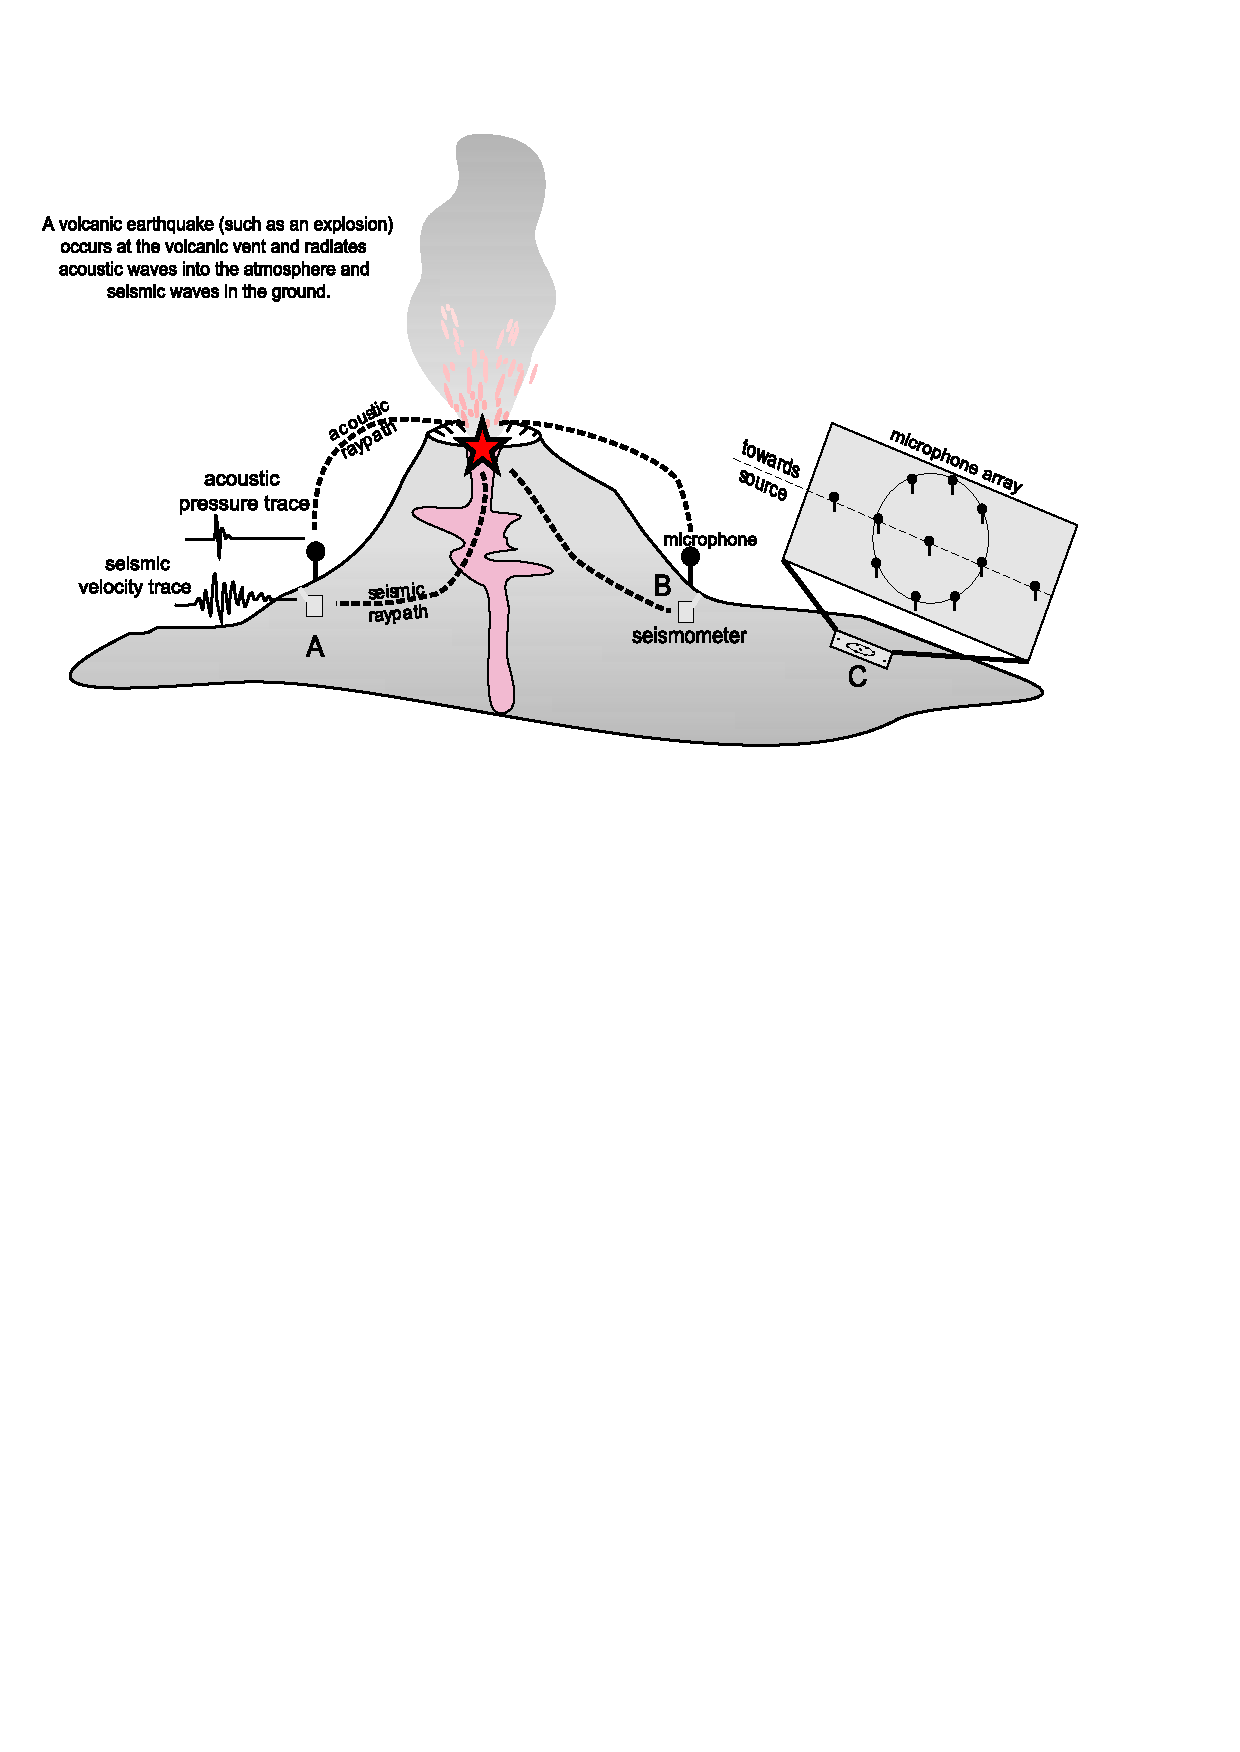
\includegraphics[width=0.9\hsize,clip=true,bb=20 470 540 770]{./2-related/figs/Cartoon2.pdf}
\end{center} 
\caption{\textbf{Sensor arrays for volcanic monitoring.}}
\label{introduction-fig-cartoon} 
\end{figure}

Networks of spatially-distributed sensors are commonly used to monitor
volcanic activity, both for hazard monitoring and scientific
research~\cite{Scarpa96}. Typical types of sensing instruments include
seismic, acoustic, GPS, tilt-meter, optical thermal, and gas flux. Volcanic
sensors range from widely dispersed instrument networks to more confined
sensor arrays. An individual sensor station could consist of a single sensor
(e.g., seismometer or tilt sensor), or an array of several closely-spaced
($10^2$ to $10^3$~m aperture) wired sensors, perhaps of different types.
Multiple stations may be integrated into a larger network installed over an
extended azimuthal distribution and radial distance ($10^2$ to $10^4$~m) from
the volcanic vent. Data from various stations may be either recorded
continuously or as triggered events and the acquisition bandwidth depends
upon the specific data stream. For instance, seismic data is often acquired
at 24-bit resolution at 100~Hz, while tilt data may be recorded with 12-bit
resolution at 1~Hz or less.

Unfortunately, the number of deployed sensors at a given volcano is usually
limited by a variety of factors, including: monetary expenses such as sensor,
communication, and power costs; logistical concerns related to time and
access issues; and archival and telemetry bandwidth constraints. Due to their
small size, light weight, and relatively low cost, wireless sensor nodes have
an important role to play in augmenting and extending existing seismic
instrumentation, providing the increased spatial resolution necessary to
support seismic applications like tomography.

\subsection{Challenges for Sensor Networks}

Wireless sensor networks have the potential to greatly enhance understanding
of volcanic processes by permitting large deployments of sensors in remote
areas. The science requirements give rise to a number of unique challenges
for sensor networks, which we outline below.

\begin{itemize}

\item \textbf{High-resolution signal collection.} Data from seismometers and
microphones must be recorded at relatively high data rates with adequate
per-sample resolution. A sampling rate of 100~Hz and resolution of 24~bits is
typical. This is in contrast to sensor networks targeting low-rate data
collection, such as environmental
monitoring~\cite{gdi-sensys04,berkeley-redwoods}.

\item \textbf{Triggered data acquisition.} Due to limited radio bandwidth
(less than 100~Kbps when accounting for MAC overhead), it is infeasible to
continuously transmit the full-resolution signal. Instead, we rely on
triggered data collection that downloads data from each sensor following a
significant earthquake or eruption. This requires sensor nodes to
continuously sample data and detect events of interest. Event reports from
multiple nodes must be collated to accurately detect \textit{global} triggers
across the network.

\item \textbf{Timing accuracy.} To facilitate comparisons of signals across
nodes, signals must be timestamped with an accuracy of one sample time (i.e.,
10~ms at 100~Hz). Data loggers generally incorporate a GPS receiver and use
low-drift oscillators to maintain accurate timing. However, equipping each
sensor node with a GPS receiver would greatly increase power consumption and
cost. Instead, we rely on a network time synchronization
protocol~\cite{rbs,ftsp} and a \textit{single} GPS receiver. However,
correcting for errors in the time synchronization protocol requires extensive
post-processing of the raw timestamps.

\end{itemize}
